\PassOptionsToPackage{hyphens}{url}
\documentclass[11pt,oneside,openright]{mpreport}
\usepackage[type=master]{wdok-title}
\usepackage[utf8]{inputenc}
\usepackage[T1]{fontenc}
\usepackage[ngerman,english]{babel}
\usepackage{textcomp}
\usepackage{mathptmx}
\usepackage[scaled=0.9]{helvet}
\usepackage{courier}
\usepackage[hidelinks]{hyperref}
\usepackage{cleveref}
\usepackage{siunitx}
\usepackage{todonotes}

\usepackage[bibencoding=auto,backend=biber,babel=other]{biblatex}
\usepackage{csquotes}

%\usepackage[style=numeric]{biblatex}
\addbibresource{main.bib}
\usepackage{mathtools}
\usepackage{svg}
\usepackage{tikz}
\usepackage{tikz-uml}
\usepackage{pgfplots}
\pgfplotsset{compat=1.14}

\DeclareMathOperator{\atantwo}{atan2}


% Examples for the definition of convenience commands
\newcommand{\package}[1]{\texttt{#1}}
\newcommand{\foreign}[1]{\emph{#1}}
\newcommand{\q}[1]{»#1«}


\newtheorem{defi}{Definition}[chapter]
\newtheorem{satz}{Satz}[chapter]
\newtheorem{bsp}{Beispiel}[chapter]

% Title Page
\title{Autonomous Driving in Urban Centers - Roundabout Monitoring}
\author{Julian-B. Scholle}

%\supervisor{Themensteller\\
%  Betreuer}


\begin{document}
\maketitle



\chapter*{Eidesstattliche Erklärung}
Ich erkläre hiermit an Eides statt, dass ich die vorliegende Arbeit selbständig und
ohne unerlaubte fremde Hilfe angefertigt, andere als die angegebenen Quellen und
Hilfsmittel nicht benutzt habe. Die aus fremden Quellen direkt oder indirekt
übernommenen Stellen sind als solche kenntlich gemacht.
Die Arbeit wurde bisher in gleicher oder ähnlicher Form keinem anderen
Prüfungsamt vorgelegt und auch nicht veröffentlicht.

\noindent Göteborg, den \today
\begin{flushright}
$\overline{~~~~~~~~~\mbox{Julian-B. Scholle}~~~~~~~~~}$
\end{flushright}


\chapter*{Acknowledgements}
Danken möchte ich außerdem besonders Associate professor Christian Berger und J. Prof Sebastian Zug, führ ihre Organisatorische und Fachliche Unterstützung während und besonders im Vorfeld dieser Abreit und
dem ``Deutschen Akademischen Austauschdienst'' - DAAD für ihre finanzielle Unterstüzung während meines Aufenthaltes in Göteborg.
Weiterhin danken möchte ich natürlich allen weiteren Kollegen aus Götborg, welche mich bei meiner Arbeit fachlich und moralisch untersützt haben.

\tableofcontents

\chapter{Introduction}

\todo{bezug auf kreisverkehre fehlt}

Das autonome Fahren und die Vernetzung von Fahrzeugen mit Ihrer Umwelt sind zusammen mit der Elektromobilität die meistdiskutierten Themen der Automobilbranche.
Zu Recht: Autonomes Fahren besitzt das Potenzial, im Mobilitätsmarkt völlig neue Strukturen entstehen zu lassen.
\footnote{\url{https://www2.deloitte.com/de/de/pages/consumer-industrial-products/articles/autonomes-fahren-in-deutschland.html} (03/09/2017)}

So ebenfalls die Technische Hochschule Chalmers welche ergänzend zu Volvos “DriveMe” Projekt das Projekt
“CampusShuttle” initiiert hat, “CampusShuttle” ist ein interdisziplinäres Forschungsprojekt der Technischen Hochschule Chalmers und der Universität Göteborg.
Das Projekt ist dabei im ReVeRe (Chalmers Research Vehicle Resource) angesiedelt. Die Vision ist dabei ein selbstfahrendes Auto zwischen den beiden Campus der Technische Hochschule Chalmers.

Dabei soll, im Rahmen des Projekts, das Fahrzeug in verschiedenen Verkehrsszenarien untersucht werden. Der Fokus liegt dabei besonders auf den Stadtverkehr, das Fahrzeug muss dabei nicht
nur in der Lage sein mit anderen Autos zu interagieren, sondern ebenfalls mit Straßenbahnen, Bussen, Fahrrädern aund allen Anderen Verkehrsteilnehmern sicher agieren. 

\section{Ausgangssituation}


\subsection{Test Platform}

\begin{figure}[!ht]
%\begin{center}
\caption{Test Platform Snowfox}
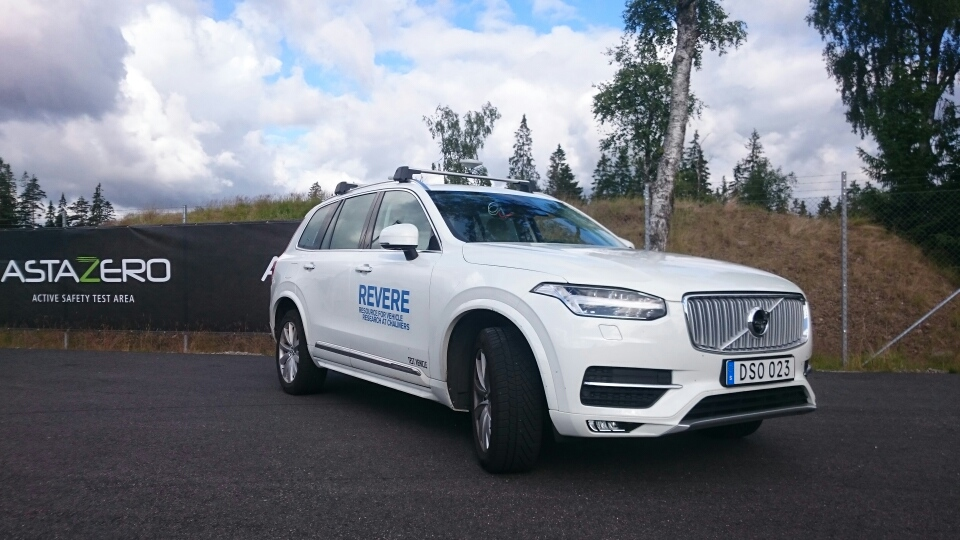
\includegraphics[width=\columnwidth]{bilder/snowfox.jpg}
\label{snowfox}
%\end{center}
\end{figure}

Die in dieser Arbeit genutze Testplatform ist ein Volvo XC90 (2015) SUV, gennate Snowfox (siehe \cref{snowfox}). Diese Testpaltform ist mit vielen Sensoren zur Umfeldwarnehmung ausgestattet.
Dazu zählen fünf Radar Sensoren, rund um das Fahrzeug. Wobei das Front Radar über eine Größere Reichweite verfügt. Sowie eine
Stereo Kamera und ein Velodyne VLP-16 LiDAR. Die Anordnung der Sensoren kann \cref{platform} entnommen werden.


\begin{figure}[!ht]
%\begin{center}
\caption{Snowfox Sensors}
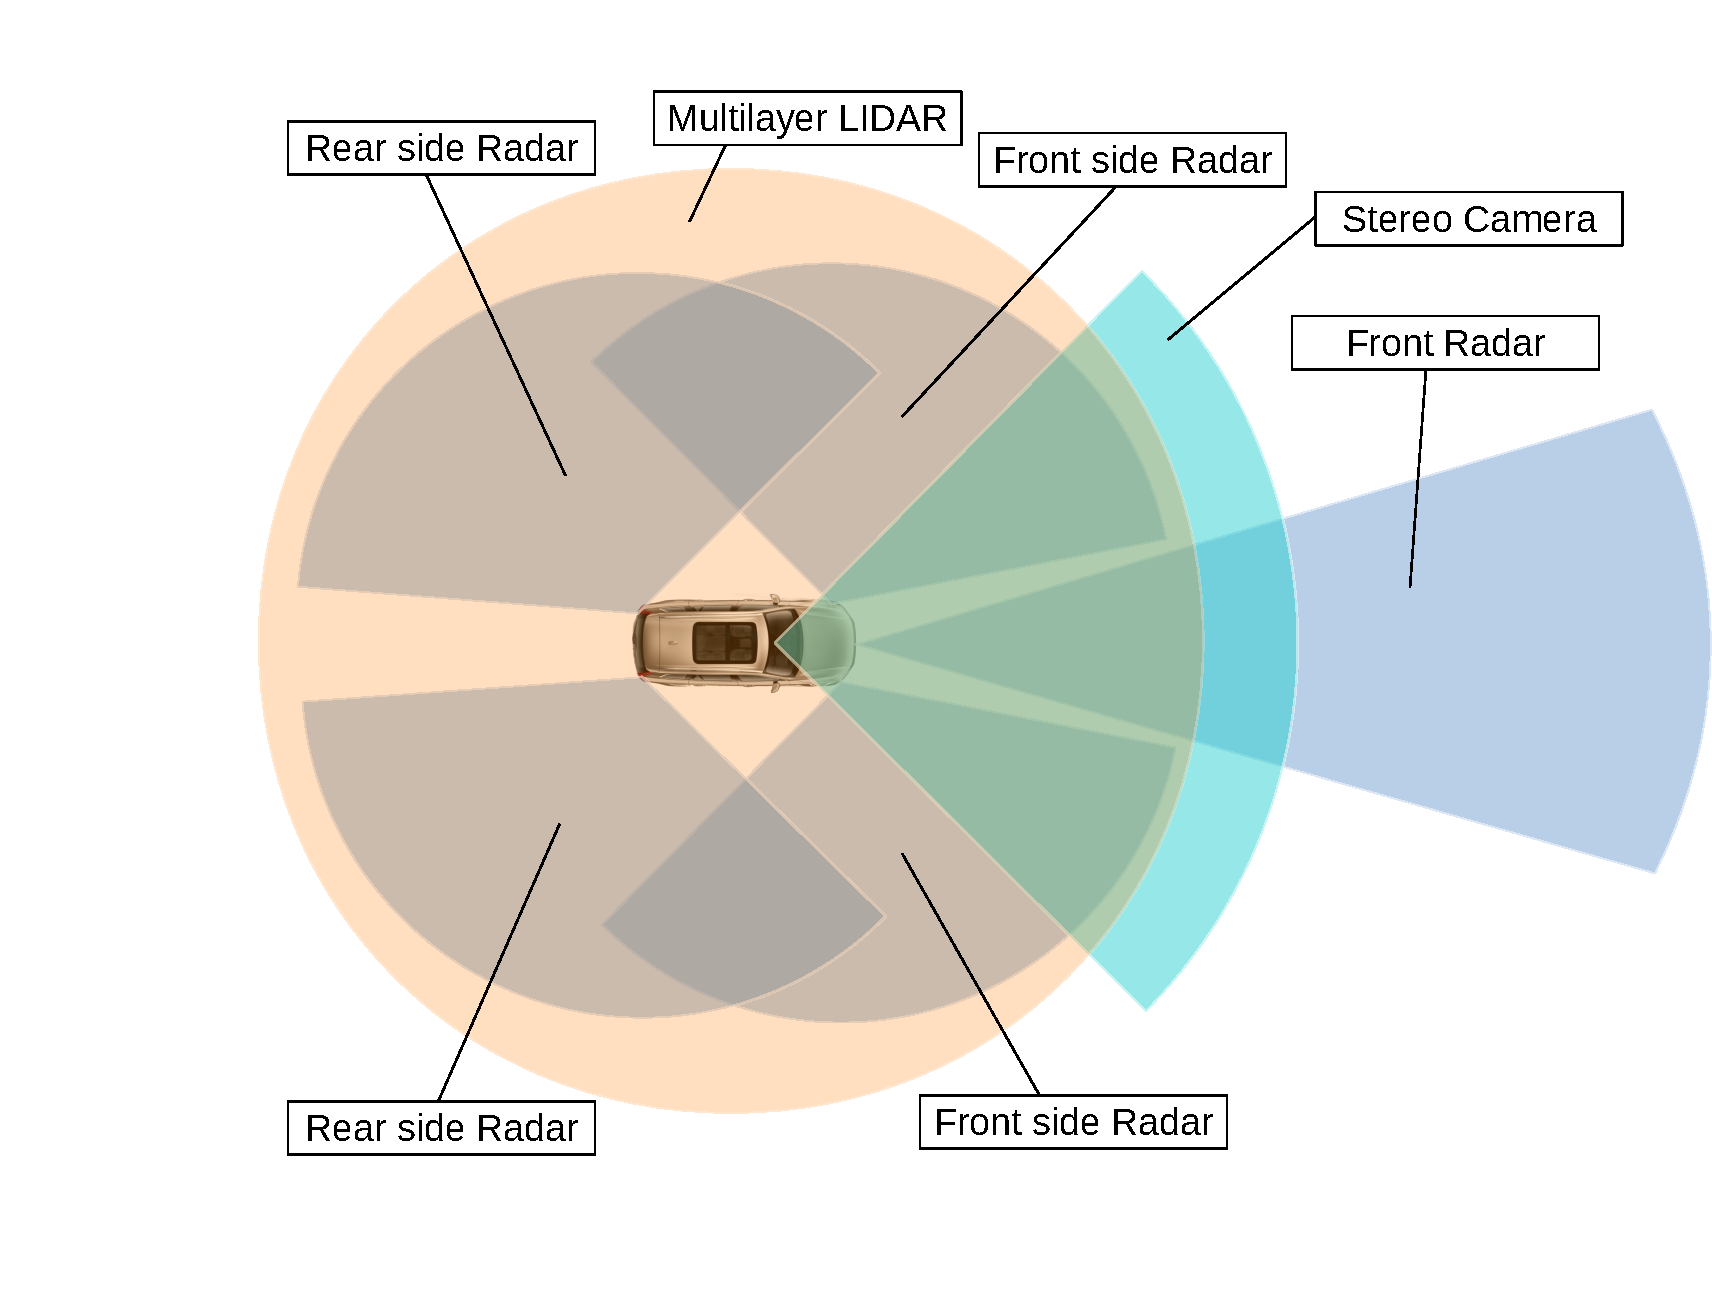
\includegraphics[width=\columnwidth]{sensors.pdf}
\label{platform}
%\end{center}
\end{figure}


Zusätlich zur Serienmäßgigen Fahrzeugsensorik (z.B. Odometer, Interialsensorik) ist im Fahrzeug ein Applanix POS LV verbaut. Zu Zeitpunkt des Verfassens dieser Arbeit war es leider noch nicht möglich auf
die Radarsensoren und die Stereokamera zuzugreifen. Daher werden im folgenden lediglich der Velodyne Lidar und das Applanix System genauer beschrieben.

\subsubsection{Velodyne VLP-16 LiDAR}
\todo{reichweitenanalyse (layer objet mit enbtfernung)}
Der Velodyne VLP-16 ist ein 360 Grad 3D Laserscannermit einer Rotationsgeschwindigkeit von 5 bis 20 Umdrehungen pro Sekunde \cite{manVEL}. Er bietet ein vertikales FOV von 30 Grad, bei 2 Grad Auflösung.
Mit einer Reichweite von 100m kann er einen Umkreis von 200m Durchmesser abdecken. Weiterhin kann der VLP-16 mit dem Applanix POS LV syncronisiert werden, was eine jitterarme Zeimessung ermöglicht.
Eine weiter Funktion des Velodyne Sensors, ist das er auf verschiedene Messimpulse reagieren kann. Durch die Auswertung des letzten Impulses statt des Stärksten Impulses ist es Möglich durch Transparent Objekte zu sehen.
Das ermöglicht uns im späteren Verlauf die Breite des Fahrzeues zu ermitteln, da der Velodyne durch die Glasfenster des Fahrzeues blicken kann.
Bei einer eingestellten Geschwindigkeit von 10Hz liefert der VLP-16 eine Auflösung von 0.2 Grad bei einer Abreichung von +-3cm. Der VLP-16 ist mittig auf dem Dach des XC90 moniert, um eine möglichst hohe Positionierung
zu erreichen, die eine Rundumsicht umd Das Fahrzeug zu erreichen. Zu beachten ist, das diese Ausrichtung für den Sensor denkbar ungünstig ist, da der Sensor ein vertikales
Sichtfeld von -15 bis +15 Grad hat. Dadurch sind nachezu alle messungen über Null grad quasi nutzlos. Der blick auf die Herstellerseite
\footnote{\url{http://velodynelidar.com/vlp-16.html} (03/09/2017)}
verrät, das Der VLP-16 aunteranderem auf die verwendung mit Drohnen hin konstuiert wurde, während der Größere HDL64E
\footnote{\url{http://velodynelidar.com/hdl-64e.html} (03/09/2017)}
explizit für den Urbanen Automotivebereich beworben wird, und über ein Sichtfeld von +2 bis -24.9 Grad verfügt und somit für die Verwendung im
Automotive bereich geeigneter erscheint. Die dabei entstehenden Probleme werden später diskutiert.



\subsubsection{Applanix POS LV}
Das POS LV ist ein kompaktes Positions- und Orientierungssystem. Es Offeriert stabile, zuverlässige und reproduzierbare Positionierungslösungen für landgestützte Fahrzeuganwendungen.
Das POS LV liefert dabei eine Inertialsensork und Odometrie gestützte Positionsmessung mit einer Genauigkeit von bis zu 0.3m (bis zu 0.035m bei verwendung von der der RTK - Korrektur).
Im weiteren Verlauf wird außerdem das vom POS LV gelieferte Heading genutzt, welches eine Genauigkeit von 0.2 Grad liefert. Auch nach ausfall des GPS-Signals kann das POS-LV durch sein
Odeomerter und der Inertialsensork eine Position liefern. Diese wird jedoch über die Zeit schlechter, so das 60Sek nach Ausfall des GPS-Signals nich eine Genauigkeit von 2.51m erwartet
werden kann.\cite{manAP}


\section{Zielsetzung}
Da das Autonome Fahren ein sehr weites, indisziplinäres thema ist, ist es Offensichtlich. das nicht alles in dieser Arbreit abgehandelt werden kann.
Im Rahmen der darpah Chalenge wurden beiteits viele Veröffentlichungen zu diesem Thema erstellet.
Was im rahmen dieser Veröffenticghungten noch nicht berhandelt wurde, sit dei Handhabung von Kreisverkehre, mit atonomen Fahrzeugen.
Ziel dieser Arbeit ist es Daher zu analysieren, welche Sensorausstattung für die beobachtung von Kreisverkehren vonnöten ist, bzw. ob die vorhandenne Sensorausstattung des ReVeRe Testfahrzeuges Snowfox
als ausreichend betrachtet werden kann.


\chapter{Related Work}

\section{Roundabouts in Law}
% In Deutschland gibt es kein Gesetzt was den genauen Konstuktion von Kreisverkehren vorschreibt.
% Stattdessen werden die Elemente der Landstraßen und Stadtstraßen in Richtlinien für die Anlage von Landstraßen (RAL) bzw.
% den Richtlinien für die Anlage von Stadtstraßen (RASt) behandelt. Diese Richtlinien sind auch für die
% Wahl einer zweckmäßigen Knotenpunktart bei der Verknüpfung von Straßen maßgebend. Für diese Abreit sind die 
% Richtlinien für die Anlage von Stadtstraßen (RASt) relevant. Die dort behandelten Abwägungsüberlegungen orientieren sich an verkehrlichen Größen, umfeldbezogenen Merkmalen,
% wirtschaftlichen Kriterien und raumordnerischen oder städtebaulichen Vorgaben. Die Richtlinien regeln auch grundlegend die entwurfstechnische und betriebliche Ausbildung von Kreisverkehren.
%
In Germany, there is no law stipulating the exact construction of roundabouts.
Instead, the elements of the rural roads and city streets are dealt with in Directives for the Design of rural roads \cite{ral13}
and the Directives for the Design of Urban Roads \cite{rast06}. These guidelines are also relevant to the choice of a convenient junction type when linking roads.
The considerations discussed there are based on traffic variables, area-related characteristics, economic criteria and spatial planning or urban planning requirements. 
The guidelines also regulate the basic design and operational formation of roundabouts.
The  Directives for the Design of Urban Roads \cite{rast06} are relevant for this dispute. Since the access the RASt ist limited, most of the information is coming from
\cite{man06} whereupon RASt is based on.
\subsection{Elements of a Roundabout}

\begin{figure}[!ht]
%%\begin{center}
\caption{Definition of individual design elements and dimensions of a roundabout \cite{man06}}
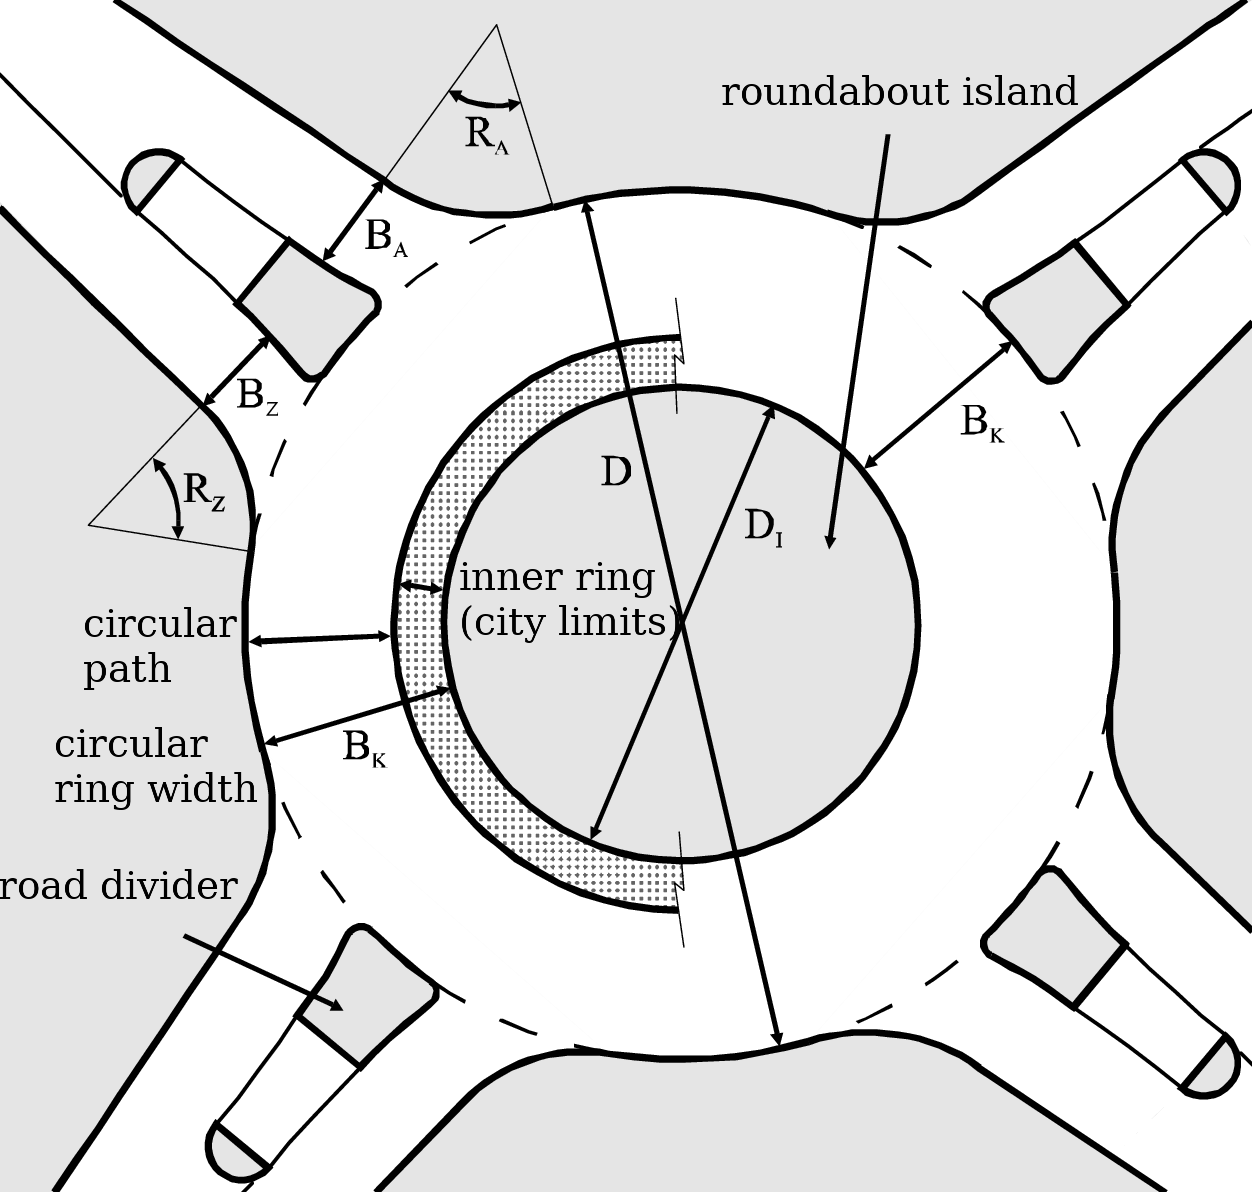
\includegraphics[width=0.7\textwidth]{bilder/kreisverkehr.png} %70% der Textbreite
\label{roundabout_parts}
%%\end{center}
\end{figure}


\begin{defi}[roundabout island]
The roundabout island is the constructional area in the middle of the roundabout, which is surrounded by vehicles.
For miniature roundabouts, the roundabout island is crossable.
\end{defi}

\begin{defi}[circular path]
%Die Kreisfahrbahn ist die Fahrbahn, die zum Umfahren der Kreisinsel
%dient. Ein ggf. vorhandener Innenring ist verkehrsrechtlich nicht Be-
%standteil der Kreisfahrbahn (VwV-StVO zu §9a V., Rn. 5).

%%TODO
The circular path is the road that serves to drive the roundabout island. An inner ring, if present, is not part of the circular path (VwV-StVO zu §9a V., Rn. 5).
\end{defi}

\begin{defi}[circular ring with ($B_K$)]
% Die bauliche Breite umfasst die Kreisfahrbahn und einen ggf. gepflasterten
% Innenring. Sie ist abhängig vom Außendurchmesser und der angestrebten
% Verkehrsführung (ein- oder zweistreifig). Die Randstreifenbreite orientiert
% sich an der maßgebenden durchgehenden Fahrbahn.
The structural width includes the circular track and a paved inner ring, if any. It is dependent on the outer diameter and the desired traffic routeing (one or two lanes). 
The edge strip width is oriented on the relevant continuous roadway.
\end{defi}

\begin{defi}[outer diameter ($D$)]
The outer diameter is measured at the outer edge of the circular ring. It is the essential measure for describing the size of the roundabout.
\end{defi}

\begin{defi}[inner diameter ($D_I$)]
The inner diameter is the diameter of the roundabout island.
\end{defi}

\begin{defi}[road divider]
% Der Fahrbahnteiler ist die baulich ausgeführte Insel zwischen Kreisausfahrt
% und -zufahrt einer angeschlossenen Straße. Er dient der Trennung der
% Kreisaus- und -zufahrten, der Führung des Verkehrs sowie den Fußgängern
% und Radfahrern als Überquerungshilfe.
%
The road divider is the structurally designed island between the circular exit
and circular driveway. It serves to separate the circular exit and circular driveway, the management of the traffic, as well as the pedestrians and cyclists as cross-bordering aid.
\end{defi}

\begin{defi}[lane width of the circular driveway ($B_Z$) and circular exit ($B_A$)]
% Die Breite der Kreiszufahrt und Ausfahrt wird am Beginn der Eckausrundung gemessen.
The width of the circular driveway and exit is measured at the beginning of the corner.
\end{defi}

\begin{defi}[Corner rounding radius ($R_Z$ and $R_A$) ]
% Dies ist der Radius der Ausrundung am rechten Fahrbahnrand zwischen 
% der Kreiszufahrt und der Kreisfahrbahn. Bei einem Korbbogen mit einer
% Radienfolge aus drei unterschiedlichen Radien ist RZ der Radius R2 des
% mittleren Bogens. Bei der Ausbildung des Fahrbahnrandes als Schleppkurve ist RZ der kleinste Radius des Fahrbahnrandes.
% 
This is the radius of the rounding at the right edge of the road between the circular driveway and the circular path.
For a elliptical arch with a radius sequence of three different radii, $R_Z$ is the radius $R_2$ of the central arc.
When the road edge is formed as a tractrix, $R_Z$ is the smallest radius of the road edge.
\end{defi}

\subsection{Types of Roundabouts}
There are several types of roundabouts, which are differentiated by the different application criteria and the partly different design principles according to the situation inside and outside built areas.
Furthermore, a division is made as a function of its size.


\subsubsection{Mini Roundabout}

\begin{figure}[!ht]
%\begin{center}
\caption{Mini Roundabout \cite{man06}}
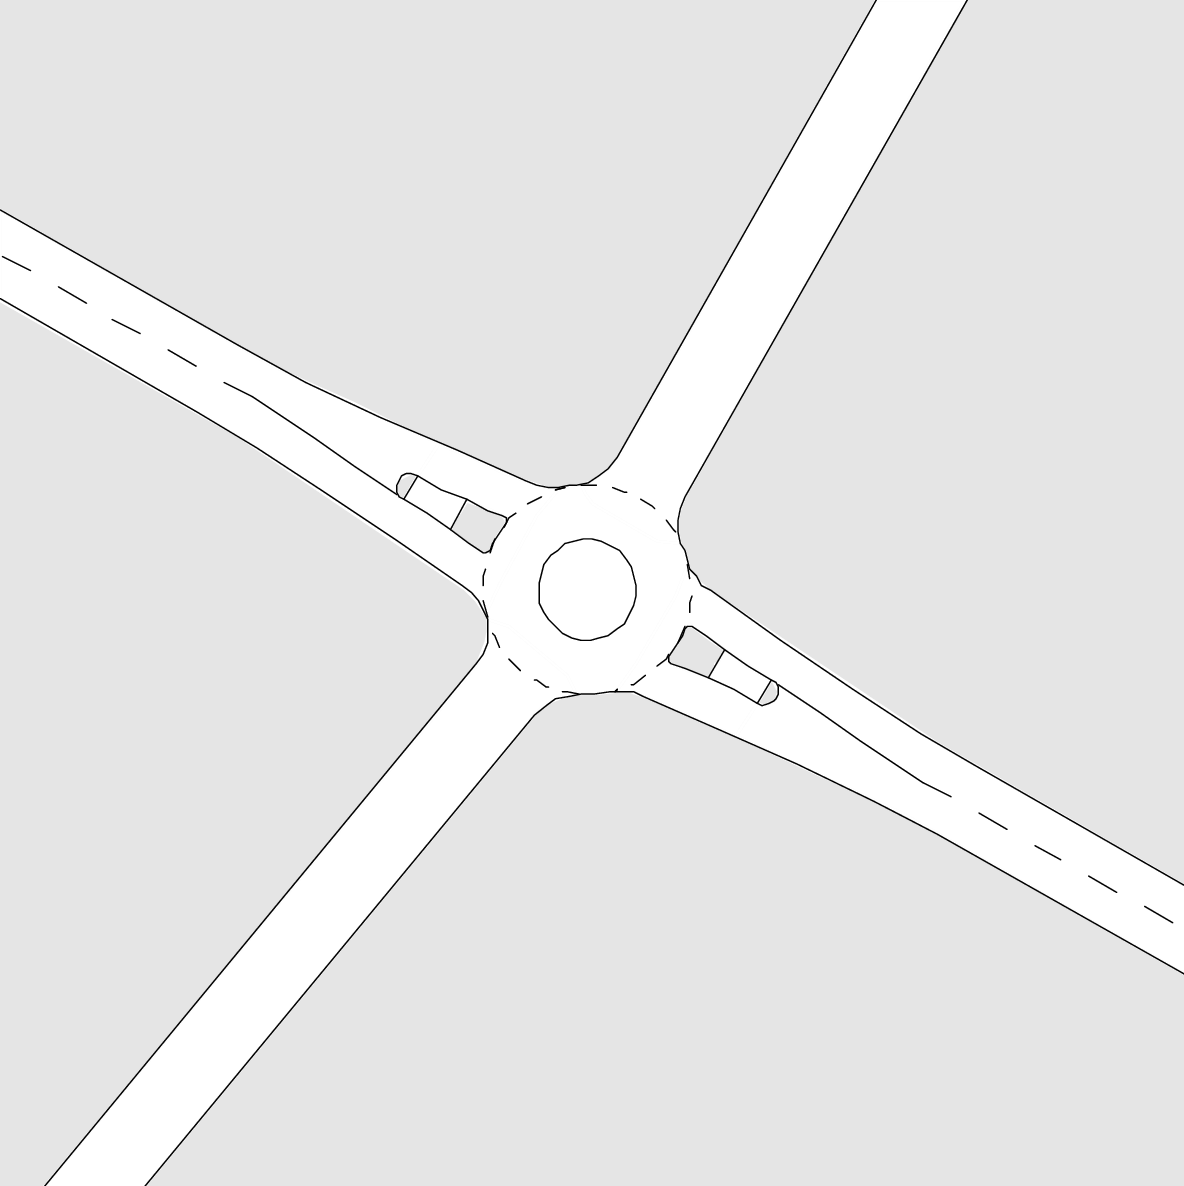
\includegraphics[width=0.5\textwidth]{bilder/mini_roundabout.png} %70% der Textbreite
\label{roundabout_mini}
%\end{center}
\end{figure}

Within built-up areas, smaller outer diameters are possible under certain conditions.
These roundabouts are called mini roundabout. The roundabout island must then be capable of being passed over.
The outer diameter should be at least 13 m, so that the circular island does not become too small.
Larger outer diameters make driving easier. Outer diameters of more than 22m, however, do not offer any transport advantages.
From an outside diameter of about 22 m, therefore, the installation of a small roundabout with 26 m is generally more convenient.
Bypasses are generally not required in the areas where mini roundabout can be used.


\subsubsection{Small Roundabout}

\begin{figure}[!ht]
%\begin{center}
\caption{Small Roundabout \cite{man06}}
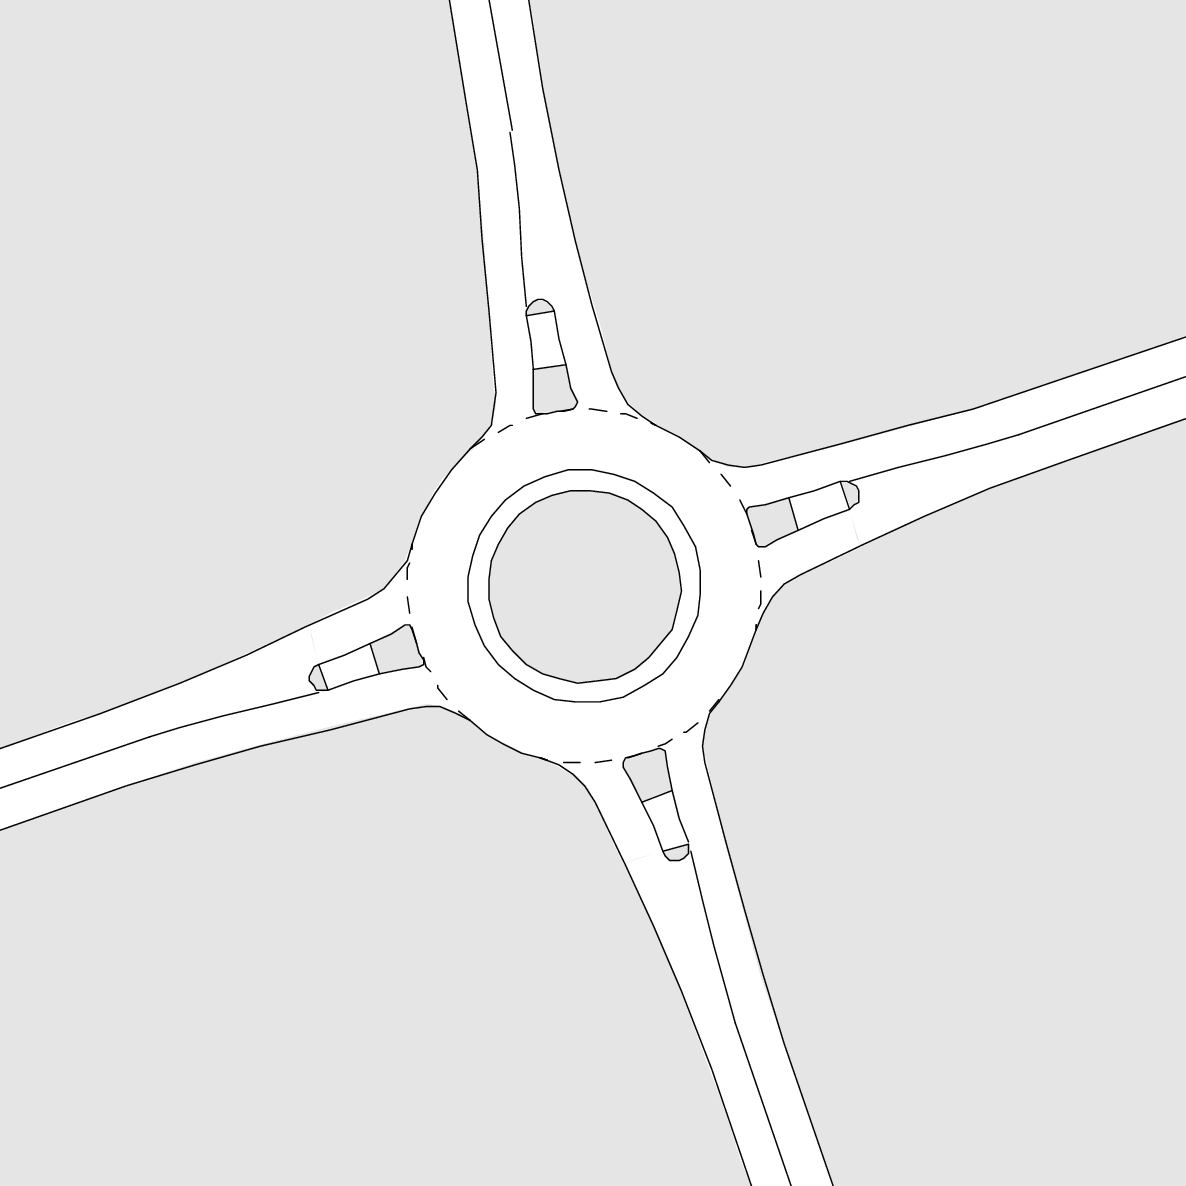
\includegraphics[width=0.5\textwidth]{bilder/small_roundabout.png} %70% der Textbreite
\label{roundabout_small}
%\end{center}
\end{figure}

The small roundabout has a single lane circular path and single lane circular driveways and exits. The roundabout island is not passable.
The outer diameter must be at least 26 m. Bypasses can be set up for driving geometric reasons or to increase performance.


\subsubsection{Two-lane Passable Roundabout}

\begin{figure}[!ht]
%\begin{center}
\caption{Two-lane Passable Roundabout \cite{man06}}
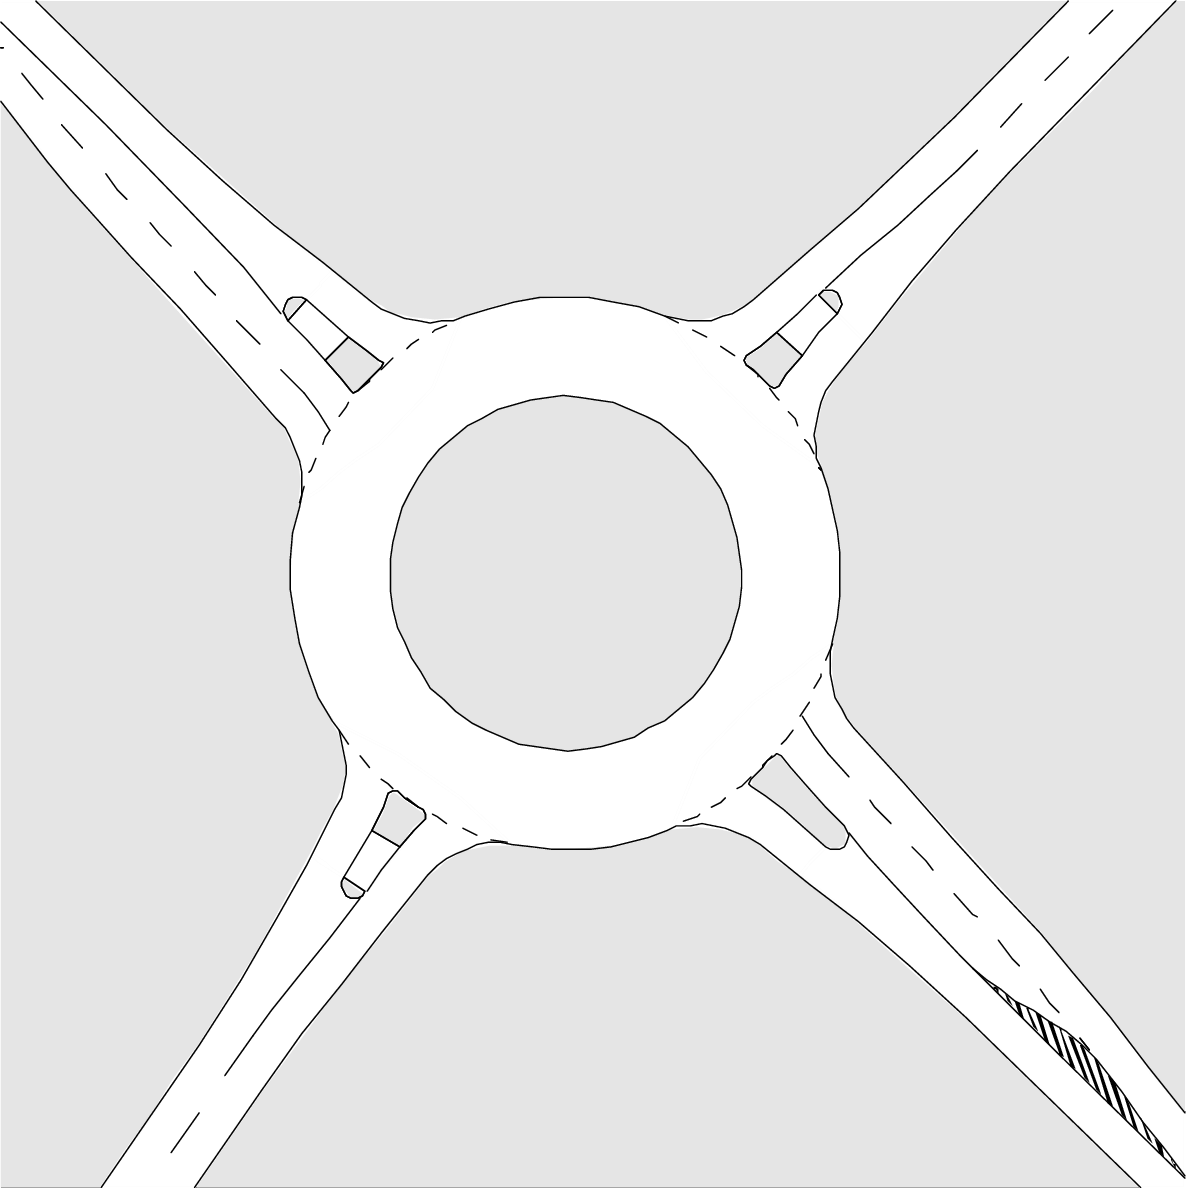
\includegraphics[width=0.5\textwidth]{bilder/twolaned_roundabout.png} %70% der Textbreite
\label{roundabout_twolaned}
%\end{center}
\end{figure}

% Reicht die Kapazität des Kleinen Kreisverkehrs nicht aus und kann diese nicht durch die Anlage von Bypässen sicher gestellt werden,
% kann die Kreisfahrbahn eines Kleinen Kreisverkehrs zweistreifig befahrbar ausgebildet werden.
% An einem solchen Kreisverkehr ist die Kreisfahrbahn so breit, dass Pkw im Kreis nebeneinander fahren können.
% Wird eine weitere Erhöhung der Kapazität erforderlich, können einzelne Kreiszufahrten ebenfalls zweistreifig ausgeführt werden,
% wenn Fußgänger und Radfahrer regelmäßig nicht zu berücksichtigen sind. Kreisausfahrten werden aus Sicherheitsgründen immer einstreifig ausgeführt.
% Aus geometrischen Gründen muss der Außendurchmesser bei zweistreifiger Befahrbarkeit mindestens 40 m betragen.
%
If the capacity of the small roundabout is not sufficient and can not be ensured by the installation of bypasses,
the circular path of a small roundabout can be designed to be two-lane driveable.
At such a roundabout, the circular path is so wide that cars can travel side by side in a circle.
If a further increase in the capacity is required, individual circular driveway can also be carried out in two lanes, if pedestrians and cyclists are not to be considered regularly.
For safety reasons, circular exits are always carried out in single lanes.
For geometrical reasons, the outer diameter must be at least 40 m for two-laned accessibility.


\subsubsection{Large Roundabout}


\begin{figure}[!ht]
%\begin{center}
\caption{Large Roundabout \cite{man06}}
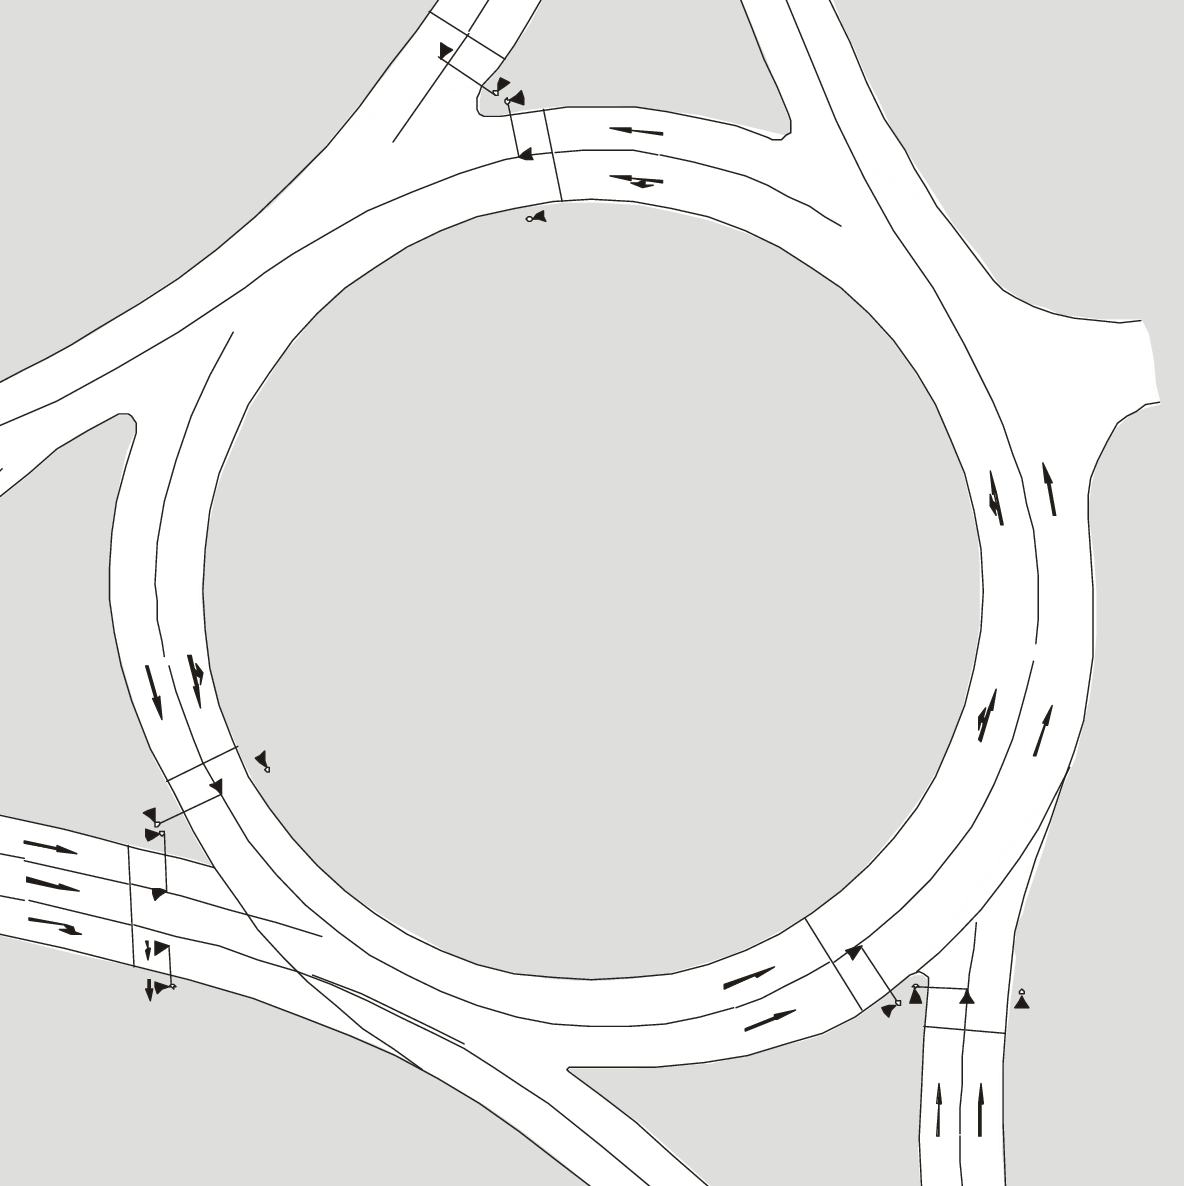
\includegraphics[width=0.5\textwidth]{bilder/large_roundabout.png} %70% der Textbreite
\label{roundabout_large}
%\end{center}
\end{figure}

%Große Kreisverkehre mit zwei oder mehreren durch Markierungen gekennzeichnete Fahrstreifen auf der Kreisfahrbahn sollen bei enger
%Abstimmung zwischen Knotenpunktentwurf und Verkehrssteuerung nur mit Lichtsignalanlage betrieben wer den.
Large Roundabouts with two or more lanes marked by markers on the circular path should be operated with a light signaling system only,
if the nodal point design and traffic control are closely coordinated.

\chapter{Methodology}
% Gefragt wird hier nach den Kriterien dafür, welche Methode für eine bestimmte Art der Anwendung geeignet ist,
% warum eine bestimmte Methode angewandt werden muss oder angewendet wird und keine andere.
% Verständnisfragen zum methodischen Weg werden hier geklärt.
% Die Methodologie ist demnach eine Metawissenschaft und somit eine Teildisziplin der Wissenschaftstheorie.
% Demgegenüber bezeichnet Methodik das Methodenwissen des Praktikers oder des Wissenschaftlers.

Im vorigen Kapitel haben wir uns die Arten von Kreisverkehren und derren Komponenten angesehen. Weiterhin haben wir die zur verfügung
stehende Testplatform und ihre Sensorik begutachtet. Dabei haben wir festgestellt, das für die Erkennung von Objekten in andren
Arbeiten häufig mehrere und teurere Sensoren kombiniert werden um ein Zuverlässiges erkennen von anderen Verkehrsteilnehmern zu gewährleisten.
In der Research Questian eins haben wir festgehalten, das wir die verwendung eines günstigen VLP-16 Sensors in einem 
Komplexen Verkehrszenario, die Verkehrsbeobachtung eines Kreisverkehrs evaluieren wollen.

Dazu wird im folgenden ein Algorithms zum erkennen und Tracken von Objekten mit hilfe des Velodyne VLP-16 vorgeschlagen
und implementiert. Die Schwierigkeit besteht dabei in der Verwendung eines Einzigen und im vergleich günstigen
Umfeldsensors, welcher offensichtlich nicht als standalone Lösung für diesen Einsatzzweck entwickelt wurde.

Dieser Sensor bietet in seiner aktuellen Anwendung in dem für diese Arbeit relevanten Bereich eine vergleichsweise
geringe Auflösung. Daher schlagen viele in ähnlichen Projekten genutzte Gradienten basierende Algorythmen im Bereich 
der Segmentierung häufig fehl. Aus diesem Grund wird für die Segmentierung eine Groundplane basierender Algorithms implementiert.

Außerdem ist es Bauartbedingt in Kreisverkehren mit bebauten Mittelinseln und Mehrspurigen Kreisverkehren nötig
Fahrzeuge über ihren Messhorizont hinaus zu verfolgen, um ein sicheres einfahren in den Kreisverkehr zu gerwährleisten.
Zu diesem Zweck wird in Section -----TODO----- ein Tracking und State Estimation Algorithms entwickelt welches dies gewähreisten soll.

Zur Evaluation dieser Algorythmen wurden mehrere Datensammlungen auf den nahe gelegenen schwedischen AstaZero \cref{astazero} Prüfgelände in Sandhult
durchgeführt, für alle nicht dort durchgeführten Expirimente werden in einer dafür erstellten Simuation durchgeführt. In dieser Simulation
wird ein Innerstätischer Kreiverkehr mit Fuß un Radweg nachgebaut, welche der Kreisverkehr auf AstaZero nicht bieten kann.

Die Evaluierung findet dabei von Hand anhand der grafisch aufbereiteten Messdaten statt. Dabei wird besonders auf False-Negativ
und False Positiv erkannte Hindernisse eingegangen. Grobe Außreißer bei der Position oder Orientierung dr Objekte werden ebenfalls verkmerkt.

Zur Evaluation der Handbarkeit des Kreisverkehrs wird außerdem eine Statemachine Implementiert welche das Fahrzeug Sicher und Unfallfrei
durch den Kreiverker bewegen soll. Dazu wird die Simulation über einen längeren Zeitraum beobachtet, und die Anzahl der eventuellen
Kollisionen notiert.

\begin{figure}[!ht]
%\begin{center}
\caption{AstaZero Proving Ground\\ \url{http://www.astazero.com/wp-content/uploads/2016/09/\%C3\%96versiktsskiss_mod.pdf} }
\includegraphics[width=\textwidth]{bilder/AstaZero.pdf}
\label{astazero}
%\end{center}
\end{figure}

% \section{Selection of Sensors}
% \section{Selection of Algorithms}
% \section{Simulation Enviroment}


\chapter{Research}
\section{Objekt Detection}

\subsection{Ground Removal}
Um in einer PointCloud Ojekte zu erkennen ist es nötig, zu wissen, welche Messungen zu Boden und welche zu Objekten gehören. Es gibt viele Möglichkeiten dieses
zu erreichen. Die Naivste Methode ist das entfernen, der Bodenplatte anhand ihrer Z-Koordinate. Diese Mehode hat allerdings viele Nachteile, zum einen muss
der LIDAR Sensor exakt gerade auf em Fahrzeug angebracht werden, zum anderen muss das Fahrzeug ein sehr steifes Fahrwerk haben, um eventuelle Neigungen des Sensors zu verhindern.
Weiterhin erlaubt dies ausschließlich die Entfernung von Palanaren Grundflächen, alo flache nicht hügelige Untergründe. Eine weitere Verbreitete Methode ist das 
Entfernen der Bodenplatte auf basis eines Statistischer mittelwertes \cite{Zhang}.  Diese Methode benötigt allerdings auch eine Kalibireirung der Sensorabstandes zum Boden.
Und die Bestimmung weiterer Schwellwerte, welche umgebungsabhäng sind. Die Votreile beider Methoden sind ihre gering nötige rechenleistung und laufzeit O(n).
Bessere Methoden wie Gradientenbasierende explansions algrythmenm benötigen einen Startpunkt der als Bodenplatte identifiziert werden kann.
Eine weitere Möglichkeit ist die Beschreibung von Objekten als Konvexe Objekte \cite{5164280}, die ebenfalls auf Basis der Gradienten beschrieben werden kann.
Vorteil dieser Methode ist das keine Initiale Position für die Bodenplatte benötigt wird.

Für unseren Anwendungsfall mit dem Velodyne VLP-16 besteht das Problem darin, dass die Auflösung des Sensor in der Höhe sehr gering ist. Abhängig von der Entfernung des 
Fahrzeuges innerhalb der benötigten Reichweite fallen nur zwei Lagen auf die Testfahrzeuge, wesshalb Gradientenbasierende Methoden hier zuverlässig versagen. Da die Gradienten zu klein sind und
die verkelinerung der nötigen Thresholds zu haufigen false Postitives führt. Die Methode des Statistischen Mittelwertes und die Methode auf basis der Z-Koordinate,
leider am Fahrwerk des Volvo XC90 SUV. Die Höhe das Fahrzeuges ändert sich aunteranderem durch veränderung des Fahrprofiles (Sport/Eco, etc.) um mehrere Zentimeter.
Auch leicht erhöhte geschwindigekiten im Kreisverkehr (ca 30 km/h) führen zu einer deutlichen Seitenneigung des Fahrzeuges. Darum wird nun eine weitere Methode vorgeschlagen.
Die Erkennung einer Grundfläche in den Messdaten. 

Für die Erknnung des Bodens gehen wir von Folgenden Annahmen aus, die Straße lösst sich approximativ als Ebene im R3 darstellen. Weiterin ist die Grundfläche die niedrigste
Fläche im Koordinatensystem. Daher wird im ersten schritt der in Polarkoordinaten vorliegende Datensatz in  in mehrere Tortenstück förmige Segmente geteilt.
Innerhalb dieser Tortenstücke wird dann eine Suche nach den 10 Messungen mit dem niedrigsten Z Wert gesucht. Die Einteilung in Segmente ist desshalb nötig
um zu verhindern, dass alle Messerte in ein einziges lokales Minima laufen. Aus diesem Vorgefilterten Messwerten werden nun für einen RANSAC drei zufällige,
jedoch nich in benachbarten Segementen liegende Messwerte, herausgesucht. Aus diesm dei Punkten wird nun eine Ebene in der Hessischen Normalform gebildet
,was eine effiziente Distanzberechnung zu anderen Punken erlaubt. Danach sammeln wir alle weiten Punkte aus unseren Minima, anahnd eines Distanzkriteriums.
Danach wird aus der Ebene und den neu Gesammelten Punkte durch einen Planefitting Algorithms [\cref{subssec:planefitting}] eine neue Ebene und derren Fehler berechnet.
Der Fehler wird über die Summe der quadratischen Abstände aller Punkte zur Ebene berechnet.

Bevor wir die Ebene jedoch als eventueller Lösungskanidat hinzufügen wird geprüft ob sich die Ebene innerhalb von einem plausiblen Parameterbereich befindet.
Dazu zählt, dass die Entfernung der Ebene zwischen 1.9m und 2.2m bewegen sollte, dies entspricht in etwa der Montagehöhe des Velodyne Sensors.

Die Anzahl an Iterationen des RANSAC ist auf 50 Begrenzt. Nach dem Durchlauf des RANSAC werden alle Punkte in der Pointcloud anhand ihrer Distanz zur Ebene als
Groundflache makiert. Als threshold wurde hier ein Wert von 0.5m genommen.


\subsubsection{Planefitting}
\label{subssec:planefitting}
Zum Planefitting einer be ne wird üblicherweise eine SVD (Singular Value Decomposition) genutzt. SVD hat eine Komplexität von $\mathcal{O}(\min\{mn^2, m^2n\}$ \cite{Holmes2007},da das Planefitting innehalb 
des RANSAC's sehr häufig mit einer großen Anzahl an Punkten ausgefürht wird, führt das Ausführen des SVD innhalb des RANSAC zu einer sehr hohen laufzeit.
Deshalb wird an dieser Stelle ein ``Linear least Squares (LLSQ)'' Algorithus mit einigen optimierungen eingesetzt. Bei der verwendung des LLSQ gilt es zu beachten,
dass nicht der abstand der Punkte zur eben optimiert wird, sondern der Abstand der Punkte zur Ebene entlang einer Achse (in unserem Fall der z Achse) siehe \cref{LLSQ_MIN}.
Das kann zu Problemen führen, wenn die Punkte weit gestreut, also weit von der Optimalen Ebene entfert sind. Da wir unsere Punkte innhalb des RANSAC allerdings anhand eines 
Distanzkriteriums vorselektieren, stellt dies kein Problem dar.

\begin{figure}[!ht]
%\begin{center}
\caption{Linear least Squares (LLSQ)  \cite{LLSQ}}
\includesvg[width=0.5\textwidth]{Linear_least_squares_min}
\label{LLSQ_MIN}
%\end{center}
\end{figure}

Die Darstellung einer Ebene in Koordinatenform sieht wie folgt aus: $ a\vec{x} + b\vec{y} + c\vec{z} + d = 0 $. Da wir eine Ebene im R3 betrachten, ist dieses Gleichungsystem überbestimmt.
Da wir unsere Ebene in Richtung der Z-Achse optimieren wollen setzten wir Parameter c auf 1 und können unser Gleichungssystem nun einfach nach z auflösen: $a\vec{x} + b\vec{y} + d = -\vec{z}$.
Die Vektoren $\vec{x},\vec{y},\vec{z}$ stellen dabei die zu fittenden Punkte dar.
In Matrixschreibweise:

\begin{align*}
X \vec{\beta} &= \vec{z}\\
\begin{bmatrix}
x_0 & y_0 & 1 \\
x_1 & y_1 & 1 \\
 & \dots & \\
x_n & y_n & 1 
\end{bmatrix} 
\begin{bmatrix}
a \\
b \\
d 
\end{bmatrix}
&= 
\begin{bmatrix}
-z_0 \\
-z_1 \\
\dots \\
-z_n 
\end{bmatrix} 
\end{align*}

Dieses Sytem hat üblicherweise keine Lösung, unser eigentliches Ziel ist jeoch auch nicht extakte lösungen für $\vec\beta$ zu finden sondern eine gute näherung $\hat{\beta}$ dafür:

\begin{align*}
\hat{\beta} = \min{(|| \vec{z} - X\vec{\beta} ||^2)}
\end{align*}

Das können wir tun indem wir unsere Gleichung mit der Transponierten unserer Punktmatrix $X$ mulltiplizieren:
\begin{align*}
(X^TX) \hat{\beta} &= X^T \vec{z}\\
\begin{bmatrix}
x_0 & x_1 & \dots & x_n \\
y_0 & y_1 & \dots & y_n \\
1 & 1 & \dots & 1  
\end{bmatrix} 
\begin{bmatrix}
x_0 & y_0 & 1 \\
x_1 & y_1 & 1 \\
 & \dots & \\
x_n & y_n & 1 
\end{bmatrix} 
\begin{bmatrix}
a \\
b \\
d 
\end{bmatrix} 
 &= 
\begin{bmatrix}
x_0 & x_1 & \dots & x_n \\
y_0 & y_1 & \dots & y_n \\
1 & 1 & \dots & 1  
\end{bmatrix} 
\begin{bmatrix}
-z_0 \\
-z_1 \\
\dots \\
-z_n 
\end{bmatrix} 
\end{align*}

Dieses Gleichungssystem könne man nun mit der Berechnung der Inverse von $(X^TX)$ auflösen. Da die Berechnung von Inversematritzen mit $\mathcal{O}(n^3)$ ebenfalls aufwändig ist,
nun ein weiterer Trick um rechenleistung zu sparen.
Nach dem Multiplizieren der Transponierten erhalten wir:
\begin{align*}
\begin{bmatrix}
\sum x_i x_i & \sum x_i y_i & \sum x_i \\
\sum y_i x_i & \sum y_i y_i & \sum y_i \\
\sum x_i & \sum y_i & N
\end{bmatrix} 
\begin{bmatrix}
a \\
b \\
d 
\end{bmatrix} 
 = 
\begin{bmatrix}
\sum x_i z_i \\
\sum y_i z_I \\
\sum z_i 
\end{bmatrix} 
\end{align*}

Gut zu sehen sind hier die Summen in den Randbereichen der Matrix X und dem Vektor $\vec{z}$. Diese können wir auf Null setzten, wenn wir alle Punkte relativ zum Mittelwert-Punkt
aller Punkte definieren, also $P_i = P_i - \overline{P}$. Nun erhalten wir:

\begin{align*}
\begin{bmatrix}
\sum x_i x_i & \sum x_i y_i & 0 \\
\sum y_i x_i & \sum y_i y_i & 0 \\
0 & 0 & N
\end{bmatrix} 
\begin{bmatrix}
a \\
b \\
d 
\end{bmatrix} 
 = 
\begin{bmatrix}
\sum x_i z_i \\
\sum y_i z_I \\
0 
\end{bmatrix} 
\end{align*}

Nun können wir d ebenfalls auf Null setzten, denn wenn alle unsere Punkte relativ zum Mittelwert-Punkt sind, dann läuft auch unsere Ebene immer durch diesen Punkt. Daher können wir 
nun eine komplette Dimension streichen:

\begin{align*}
\begin{bmatrix}
\sum x_i x_i & \sum x_i y_i \\
\sum y_i x_i & \sum y_i y_i
\end{bmatrix} 
\begin{bmatrix}
a \\
b 
\end{bmatrix} 
 = 
\begin{bmatrix}
\sum x_i z_i \\
\sum y_i z_i
\end{bmatrix} 
\end{align*}

Das Gleichungssystem können wir nun einfach mit der Cramer's rule lösen
\begin{align*}
D &= \sum x_i x_i \cdot \sum y_i y_i - \sum x_i y_i \cdot \sum x_i y_i \\
a &= \frac{\sum y_i z_i \cdot \sum x_i y_i - \sum x_i z_i \cdot \sum y_i y_i }{D}\\
b &= \frac{\sum x_i y_i \cdot \sum x_i z_i - \sum x_i x_i \cdot \sum y_i z_i }{D}\\
\vec{n} &= [a, b, 1]^T
\end{align*}
Dabei gibt es zu beachten, dass die Determinante nicht Null oder nahe Null sein darf.
Da der winkel zwischen dem Fahrzeug und der Ebene jedoch immer nahe 90 Grad liegt, ist die Determinante typischweise sehr groß. 
Sollte die Determinante doch nahe 0 (nicht gleich 0) sein, wird die Berechnung trotzudem durchgeführt, da dies auch zu einem 
großen Fehler im Fitting führt. Dies ist an dieser Stelle erwünscht, da der RANSAC ungeültige Ebenen anhand des Fehlers ausssortiert.
Ist die Determinante extakt Null, wird die Berechnungstatdessen mit einem kleinen Wert für D fortgesetzt.

Aus dem Normalenvektor $\vec{n}$ und dem Mittelwert-Punkt $\overline{P}$ können wir nun wieder die Hessische Normalenvektor bestimmen.

Letztendlich haben wir so den Algorithms von $\mathcal{O}(m^2n) $ auf $\mathcal{O}(n) $ runterbrechen können.

\subsection{Clustering}
In aktuellen Abreiten mit 3D-LIDAR Daten werden de Daten haufig als erstes in eine Heightmap projeziert \cite{Zhang,Himmelsbach2009,Li2016}.
Danach werden direckt benachbarte Messungen mit ähnlichen Messwerten zusammengefasst. Alternativ werden die Messungen auch anhand eines Distanzkritterums 
zusammengefasst. Erstere Methode hate den Nachteil, dass einzelne Ausreißer dazu führen, das das Objekt in mehrer Cluster zerfällt.
Letztere wird meißt mit einem KD-Tree oder einer ähnlichen Datenstrucktur kombiniert, welche typischerweise hohe Kosten für die Erstellung verursachen.
Da der Baum nach jeder 360 Grad messung neu Aufgebaut werden muss ist das Problematisch

Hier wird eine Methode vorgeschlagen welche die Vorteile beider Methoden kombiniert. Dauzu ist es nötig zu wissen, wie die Daten von der OpenDAVINCI 
Middleware geliefert werden. Das OpenDAVINCI auf der Übertragung der Daten mit UDP Multicast setzt, werden die Daten in einer Kompakten form übertragen, welche in einen einzigen
UDP Frame passt.\\
\begin{center}
\begin{tikzpicture} 
\umlclass{CompactPointCloud}{
startAzimuth : float \\
endAzimuth : float \\
entriesPerAzimuth : uint32 \\
distances : byte[]}
{getStartAzimuth : float\\
\dots}
\end{tikzpicture}
\end{center}
Dabei wird von einer konstanten Drehrate des Sensors ausgegangen, was in einer äquidistanten der Messwerte resultiert. Die Anzahl der Messungen pro Azimuth
wird in entriesPerAzimuth festgehalten und entspricht für den Velodyne VLP16 16. Um nun an die Eigentlichen Messwerte zu kommen müssen jeweils zwei distance Werte zu
einem Unsigned 16Bit Integer umgewandelt werden, welcher dann die Messung in cm enthält. Jeweils 16 dieser Werte ergeben dann einen Messframe in dem der Polarwinkel
auf einen Bereich zwischen -15 und +15 abgebildtet werden muss. Nachdem die sphärische Daten wiederhergestellt wurden, werden diese In Kartesische umgewandelt und
in eine Punkt Datenstruktur gespeichert. 

\begin{center}
\begin{tikzpicture} 
\umlclass{Point}{
azimuth : float \\
measurement : float \\
visited : bool \\
isGround : bool \\
point : vector3f \\
}
{getAzimuth : float\\
\dots}
\end{tikzpicture}
\end{center}

Diese wird wiedrrum in ein Statisches 2 Dimensionales Array Gespeichert: Points[2000][16]. Die Reihenfolge der Daten wird dabei beibehalten.
Diese Datenstruktur stellt nun im weiteren verlauf unsere Pointcloud dar.

Auf dieser Basis wird nun ein DBSCAN (Density-Based Spatial Clustering of Applications with Noise) \cite{DBSCAN} ausgeführt. Der DBSCAN Algorithms hat dabei folgende Vorteile.
Im Gegensatz beispielsweise zum K-Means-Algorithmus, muss nicht im vornherein bekannt sein, wie viele Cluster existieren. Der Algorithmus kann Cluster beliebiger Form 
(z.B. nicht nur kugelförmige) erkennen. Das macht den DBSCAN damit für uns zu optimalen Kandidaten. DBSCAN selbst ist von linearer Komplexität.
Die meiste Rechenzeit wird jedoch überlichweise durch die Nachbarschafts berechnung verursacht. Genau hier setzen wir an, anstatt der Bereichsanfrage über eine Baum-Struktur
nutzten wir aus, dass Messungen in einer kleinen Nachbarschaft einen ähnlichen Azimuth Winkel haben. Dazu untersuchen wir für jeden Messwert jeweils zwei weitere Einträge nach links
und rechts in unserem Array. Effektiv müssen wir daher $5 \cdot 16 = 80$ werte Überprüfen. Die Laufzeit der Bereichsanfrage kann deshalb in linearer Komplexität durchgeführt
werden. Alle Messwerte die Zuvor als Grund Klassifiziert wurden, werden bei der Berchnung übersprungen, zusätzlich entfällt der Aufbau eines KD-Trees. 


\subsection{Tracking}
Das Tracking ist in zwei Abschnitte unterteilt. Dem Tracking der Cluster vom DBSCAN und dem Erstellen und Tracken von Hindernissen.

\subsubsection{Cluster Tracking}
Für das Tracking der Cluster nehmen wir an, dass sich Objekte von Zeitschritt zu Zeitschritt nur geringefügig bewegen, weiterhin
ändert sich die Form der Cluster ebenfalls nur leicht. Das ist wichtig, da die Position eine Clusters durch einen Mittelwertpunkt definiert ist.
Das Tracking wird im R2 durchgeführt. Im Initialen Schritt wird jeden Cluster eine aufsteigende ID zugerordnet.
In jedem weiteren Schritt wird jedem neuen Cluster die ID des alten Clusters zugeordnet welcher über die Zeit hinweg die geringste Entfernung aufweißt.
Fur diese Entfernung gibt es eine großzügige obere Schranke von 3m, Cluster die nicht innerhalb in dieser Grenze sind erhalten eine neue ID.
Das führt dazu, dass mehreren Cluster die selbe ID zugeordnet werden kann, das ist wichtig, da Objekte manchmal in mehrere Cluster zerfallen.

\subsubsection{Object Tracking}
Basis für das Objekt Tracking sind die zuvor gtrackten Cluster. Im Initialen Schritt werden aus allen Cluster mit der Selben IDs Objekte gebildet.
In jeden weiteren Schritt werden Alle Cluster mit der zuvor gleichen ID zum updaten der Objekte genutzt. Aus Clustern mit neuen IDs werden neue Objekte gebildet.

Der vorerst wichtigste Schritt beim Updatevorgang ist die berechnung der Bewegungsrichtung eines Objektes, da folgende Berechnungen auf dieser basieren.
Bei der Berechnung der Bewegungsrichtung ist zu beachten, dass die Bewegung des eigenen Fahrzeuges herausgerechnet werden muss.
Dazu werden die Positionsdaten des Applanix POS-LV genutzt. Da sowohl die Positionsdaten des Applanix Systems, als auch die Erkannte Postition des Fahrzeuges Fehlerbehaftet sind,
wird die Bewegungrichtung nur bei einer minimalen Bewegung von 2m geupdatet.

\begin{align*}
\Delta x &= P_x(t) - P_x(t_{-2m}) + \Delta C_x\\
\Delta y &= P_y(t) - P_y(t_{-2m}) + \Delta C_y\\
\theta &= \atantwo(\Delta y,\Delta x)
\end{align*}

mit $P$ - Postition des Objekts, $C$ - Position des eigenen Fahrzeuges

Das Ergebnis kann in \cref{obst_rot} betrachtet werden. Gut zu erkennen ist, dass die Bewegungsrichtung (Pfeil) nicht mit der Ausrichtung des Objekte (schwarz) übereinstimmt,
die Boundingbox jedoch korrekt ausgerichtet ist. Wie diese Berechnung zustande kommt wird im folgenden geklärt.

\begin{figure}[!ht]
%\begin{center}
\caption{Obstacle Movement}
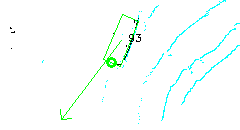
\includegraphics[width=0.5\textwidth]{bilder/obst_rot.png}
\label{obst_rot}
%\end{center}
\end{figure}

Basierend auf der Bewegungrichtung wird nun die Ausrichtung des Fahrzeiges berechnet. Dazu werden alle dem Objekt zugewiesenden Cluster zusammengefasst und um $-\theta$ gedreht.
Danach wird das Objekt wird in 3 gleich große Segmente unterteilt (\cref{obst_devide}).

\begin{figure}[!ht]
%\begin{center}
\caption{Obstacle Cutting}
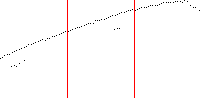
\includegraphics[width=0.5\textwidth]{bilder/obst_devide.png}
\label{obst_devide}
%\end{center}
\end{figure}

Weiterhin wird bestimmt ob sich das Objekt oberhalb oder unterhalb der x-Achse befindet. Dies ist wichtig, da wir wissen müssen, welche seite des Objekts wir messen.
Befindet sich das Objekt aso unterhalb der x-Achse wird im nächsten Schritt der y-Wert maximiert, befindet es sich oberhalb, wird er minimiert.
Im folgenden gehen wir davon aus, dass sich das Objekt unter der x-Achse befindet. Deshalb maximieren wir nun im linken und rechten Segment des Geteilten
Hindernises die y-Werte. Die Unterteilung in 3 Segmente ist nötig um zu verhindern, das bei perfekt wagerechte ausgerichteten Objekt beide Maxima in den selben Punkt laufen.
Mit diesen Punkten $(\vec{R};\vec{L})$ wird nurn eine korrektur der Drehung des Objektes berechnet:

\begin{figure}[!ht]
%\begin{center}
\caption{$\theta$ - Correction}
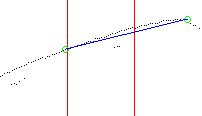
\includegraphics[width=0.5\textwidth]{bilder/obst_devide_angle.png}
\label{obst_correction}
%\end{center}
\end{figure}

\begin{align*}
\Delta x &= R_x - L_x\\
\Delta y &= R_y - L_y\\
\theta_{correction} &= \atantwo(\Delta y,\Delta x)
\end{align*}

Nach Anwendung der Korrektur wird die größe des Hindernises berechnet. Dazu werden die maximalen und minimalen x und y Werte herangezogen.
Mit diesen Werten wird nun über die Zeit ein auf 0.5m gerundetes Histogram für die Länge und Breite des Hindernises aufgebaut.
Anhand diesem wird dann der warscheinlichste Wert ausgewählt. Dadurch ändert sich die Größe des Hindernisses zu begin häufiger,
bevor die Größe auf einen stabilen wert konvergiert.Da die größe des Objekts zu begin sehr klein sein kann, 
gibt es für beide Werte einen unteren Grenzwert. Messerte für ein Beispielobjekt sind in \cref{obst_hist} zu sehen.
\begin{figure}[!ht]
  %\addcontentsline{lof}{figure}{LaTeX--Strukturelemente}
%\begin{center}
\caption{Object Size Histogram}
\begin{tikzpicture}
\begin{axis}[ybar interval, ymax=366,ymin=0, minor y tick num = 3,
width=0.55\textwidth,
height=0.6\textwidth]
\addplot coordinates { (1.0, 29) (1.5, 58) (2.0, 366) (2.5, 35) (3.0, 3) (3.5, 1) };
\end{axis}
\begin{axis}[ybar interval, ymax=318,ymin=0, minor y tick num = 3,
width=0.55\textwidth,
height=0.6\textwidth,
at={(0.50\textwidth,0)}]
\addplot coordinates { (2.0, 7) (2.5, 6) (3.0, 9) (3.5, 2) (4.0, 64) (4.5, 84) (5.0, 318) (5.5, 3) (6.0, 2) (6.5, 2) };
\end{axis}
\node at (0.21\textwidth,0.5\textwidth) {width};
\node at (0.7\textwidth,0.5\textwidth) {length};
\end{tikzpicture}
\label{obst_hist}
%\end{center}
\end{figure}

Leicht zu sehen wird für das Object eine breite von 2m und eine Länge von 5m berechnet. Das Objektist in diesm Fall ein Volvo S60, welcher Außenmaße von ca. 1.9m und 4.6m hat,
womit die Abweichungen sich korrekt innerhalb, der Rundung der Werte befinden. Für die Nachfolgende filterung der Messwerte mit Hilfe eines Kalman filters, wurd nun
die Position des Fahrzeuges aus dem Mittelpunkt der Boundingbox bestimmt.

Die für die Berechnung der Bewegungsrichtung genutzte Position ist jedoch eine andere, da die so eben berechnete Position zu diesem Zeitpunkt noch nicht zur verfügung steht und
die Position kurz nach der Initialen erkennung durch die häufigen Größenändrungen sehr instabil ist. Deswegen wird als Position immer die maximale x-Koordinate der Cluster gesnutzt.
Diese Postition kann ebenfalls in \cref{obst_rot}, als grüner Punkt begutachtet werden.
Da $\theta$ im initialen Zeitschritt Null ist, entpricht dies der globalen Maximalen x-Koordinate des Clusters. Dies Führt dazu, das wir im Initialen Zeitschritt annhemen, dass sich das Objekt
in die positive x-Richtung bewegt. Bei Objekten bei denen das nicht der Fall ist, führt das zu einem kurzzeitigen oszillieren der Orientierung, welche sich jedoch über die Zeit schnell stabilisiert.


Der eine oder ander möge sich wundern warum die Boundingbox so aufwendig berechnet wurde. Eine Einfache Art und weise eine Boundingbox für die Objekte zu berechnen wäre die berechnung
der Minimum Boundingbox über die konvexe Hülle, so wie es in vielen Anderen Arbeiten gemacht wird \cite{Zhang,Himmelsbach2009}. Die Minimum Bounding box liefet jedoch unter umständen nicht das gewünschte
ergebnis, zum einen hat die immer nur die größe der aktuellen Messung und zum anderen kann sie eine falsche Orientierung liefern, wie in \cref{min_box} zu sehen.

\begin{figure}[!ht]
%\begin{center}
\caption{Error with minimum Boundingbox \cite{Himmelsbach2009}}
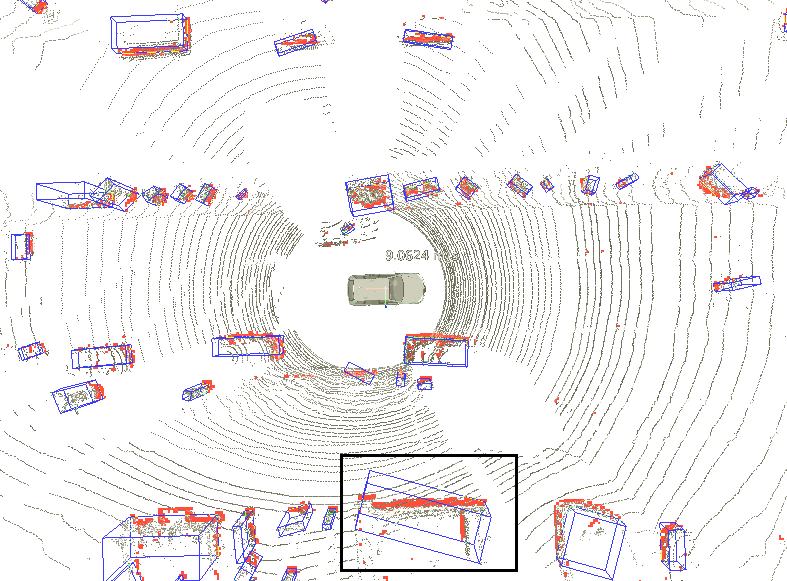
\includegraphics[width=\textwidth]{bilder/min_bound.png}
\label{min_box}
%\end{center}
\end{figure}

Da die orientierung und Postition der Objekte jedoch als eingang für den nachfolgenden Kalmanfilter genutzt wird, welcher sehr sensible auf falsch Orientierungen reagiert, wurde eben jeder Algorithmus
entwickelt.




\subsection{Classification}

Die Klassifizierung der Objekte finedt anhand ihrer Größe statt, es findet keine Klassifizierung nach bewegten und unbewegten Objeten Stadt.
Unterschieden werden lediglich Fußgänger, Radfahrer, und Fahrzeuge, und Sonstige. Als Klassifizierungs kritterien werden dabei unter anderem, die Größe der Cluster und ihre Geschwindigkeit genutzt.
Objekte die eine Größe von 2x1.5m überschreiten werden dabei als Fahrzeug Klassifiziert, Objekte die kleiner als 1x1m sind werden als Fußgänger klassifiziert. Alles dazwischen wird als Radfahrer klassifizierfiziert.
Weiterhin wird andhand der Geschwindigekeit eine Plausibilitätstest durchgeführt. So darf eine Fußgänger eine Geschwindigekeit von 10km/h nicht überschreiten und die Maximalgeschwindigkeit dür einen 
Radfahrer bertägt 30km/h. Da für Fahrzeuge keine sinnvolle geschwindigkeitsgrenze angenommen werden kann, wir an ihrer stelle die Änderung der Orientierung genutzt. Als Maximale Drehrate wird
eine Messung von 0.3 rads/sec aus \cite{Kelly1994} angenommen. Da der Wert eine Obere Grenze darstellen soll nehmen wir einen etwas höheren  Wert von  0.3 rads/sec an.



\subsection{State Estimation}

Nachfolgende des Trackings wird auf den Erkannten Objekten eine Zustandschätzung durchgeführt. Dies ist nötig, da Objekte während der Fahrt verdenkt werden können,
sei es durch andere bewegte Objekte oder Gebaüde. Eine schätzung des Zustandes über den Erkennungshorizont hinaus erlaubt es uns eine Aussage über die Position von
Objekten zu treffe, welche im Moment nicht sichtbar sind. Weiterin erlaubt es auf einfache Weise zeitweise nicht erkannte Objekte wiederzuerkennen, also dem Objekt
die gleich ID zuzuweisen wie zuvor. 

Aus dem zuvor durchgführten Tracking können wir die Aktuelle Position, Geschwindigekeit, Drehung und Drehgeschwindigkeit erhalten. 
Für eine Zustandschätzung mit den für Fahrzeuge üblichen Bicycle Model fehlen und Angangen über den Radstand und Gewicht des Fahrzeues.
Daher müssen wir uns auf ein relativ Einfaches ``Constant Turn Rate and Velocity'' Model beschränken. Dies erlaubt es uns allerdings das gleiche
Model für alle Klassen von Objekten zu nutzten. Da dieses Model ebenfalls auf Fußgänger und Radfahre angewendet werden kann.

\subsubsection{Constant Turn Rate and Velocity Model}
Der Zustandvektor \cite{Schubert2008} des CTRV- Modells sieht wie folgt aus:
\begin{align*}
\vec{x}(t) &=
\begin{bmatrix}
x & y & \theta & v & \omega
\end{bmatrix}^T\\
x &\text{ - Y Axis}\\
y &\text{ - X Axis}\\
\theta &\text{ - Object Yaw Angle}\\
v &\text{ - Object Velocity}\\
\omega &\text{ - Yaw Rate}
\end{align*}

Die Dynamikmatrix erhalten wir durch eine nichtlinieare Zustandsübergang:

\begin{align*}
\vec{x}(t + T)=
\begin{bmatrix}
\frac{v}{\omega} (-\sin(\theta)) + \sin(T \omega + \theta) + x(t) \\
\frac{v}{\omega} (\cos(\theta)) - cos(T \omega + \theta) + y(t) \\
\omega T + \theta\\
v\\
\omega
\end{bmatrix} 
\end{align*}

% Da es sich beid er Dynamikmatrix um einen nichtlinearen Zustandsübergang handelt benötigen wir noch die Jacobi Matrix.
% Die Matrix wure mit Sympy generiert, und auf Grund ihrer Größe eingekürzt.
% 
% 
% \begin{align*}
% J(\vec{x})=
% \begin{bmatrix}
% 1 & 0 & \frac{v}{\omega} (-\cos(\theta)) + \cos(T \omega + \theta)& \dots & \dots \\
% %\frac{1}{\omega} (-\sin(\theta)) + \sin(T \omega + \theta)&
% %\frac{Tv}{\omega} \cos(T \omega + \theta) - \frac{v}{\omega^2}(-\sin(\theta) + \sin(T\omega + \theta) 
% 0 & 1 & \frac{v}{\omega} (-\sin(\theta)) + \sin(T \omega + \theta)& \dots & \dots \\
% 0 & 0 & 1 & 0 & T\\
% 0 & 0 & 0 & 1 & 0\\
% 0 & 0 & 0 & 0 & 1
% \end{bmatrix} 
% \end{align*}

\subsubsection{Prediction}
Befindet sich ein Objekt innerhalb der Rechihweite des Velodyne Sensors und wird im Darauffolgenden Zeitschritt nicht erkannt,
wird der Prediktionsschritt des Kalman filter weiterhin ausgeführt. Dies geschieht solange die Unsicherheit der Position einen gewissen Schwellwert üerschreitet.
Sobald das Clustertracking dann ein neues Objekt detektiert, dem keine Bisher bekannte ID zugewiesen werden kann, wird die Postion mit allen Onjekten in der Prediktionsphase
abgeglichen. Befindet sich das neue Objekt nahe an der predizierten Position wird der Cluster dem Onjekt zugewiesen, und der Korrekturschritt des EKF durchgeführt.







\section{Mapping}
\subsection{OpenDAVINIC Map}
\subsection{Simplification}




\chapter{Evaluation}

\section{Simuation}
\section{Real Measurements}
\chapter{Conclusions}
Kann in mehrere Unterkapitel gegliedert werden\\\\
Greift Thesen oder Fragestellungen aus der Einleitung wieder auf\\\\
Fasst die Arbeit knapp und prägnant zusammen\\\\
Ordnet die Ergebnisse in Gesamtzusammenhänge ein\\\\
Zieht Schlussfolgerungen aus den erarbeiteten Ergebnissen\\\\
Kann auch eigene Bewertungen oder Meinungen enthalten\\\\
Gibt eine Ausblick auf mögliche Konsequenzen oder notwendige weitere zu lösende Probleme
\chapter{Future Work}

\printbibliography

\end{document}          
